\chapter{Lecture 10}

%--- 信息 ----
\begin{center}
    讲师:王立威 \qquad
    课程时间:25.Apr.22nd\qquad 
    笔记:25.June.9th
\end{center}

\bigskip

关于编码的部分就到此结束,我们转而关注信道传输中的根本问题. 这章的核心是信道容量(channel capacity). 先总结一下信道通信的基本框架,图示如下:
\begin{figure}[H]
    \centering
    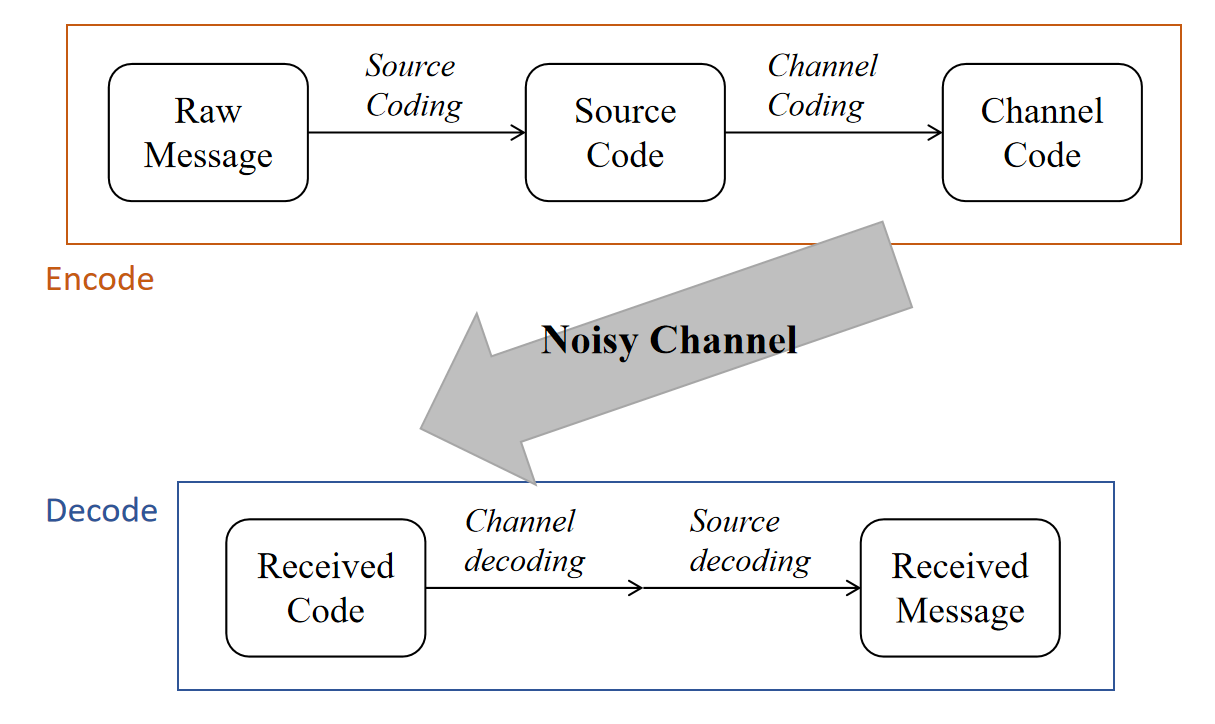
\includegraphics[width=.95\textwidth]{images/c10_1.png}
    \caption{信道通信的图示}
\end{figure}

如何刻画一个含噪的信道呢?我们将信源的消息看作随机变量$X$,通过信道后的信息为$Y$,那么含噪信道在意义上完全可以由似然(条件概率)$\Pr[Y|X]$决定(一下可能使用$P(Y|X)$代替$\Pr[Y|X]$).

在这个模型的基础上,当给定一个含噪信道$P(Y|X)$后,接收方能够接受到有多少有关$X$的“信息”.  如果我们单纯用信息熵来刻画是不够合理的:
\begin{proposition}
    存在含噪信道$P(Y|X)$使得$H(Y) > H(X)$.
\end{proposition}

这是因为接收方可能收到了很大一部分来自噪声的信息,而非来自$X$的信息,故我们再次强调该信息一定是关于$X$的. 自然我们应该使用互信息而非信息熵来刻画,即使用$I(X;Y) = D(P_{X,Y} \| P_X P_Y)$. 

因此延伸出信道容量的定义:
\begin{definition}[信道容量]
    对于一个含噪信道$P(Y|X)$,其\textbf{信道容量}(channel capacity)定义为 
    \[
    C:= \max_{P_X} I(X;Y)
    \]
\end{definition}

可以看出信道容量的物理意义是有效信息最高传输速率. 为加深理解,来看几则例子. 
\begin{example}
    $X,Y$均取值于$\{0,1\}$,若信道是无噪声的,即似然如下,求容量.
    \[
    \begin{array}{c|c|c}
        P(Y|X) & X=0 & X=1 \\ \hline 
        Y=0 & 1 & 0 \\ \hline 
        Y=1 & 0 & 1        
    \end{array}
    \]
\end{example}
\begin{solution}根据定义有
    \[
        C = \max_{P_X} I(X;Y) = \max_{P_X} H(X) = 1 \ \text{bit}
    \]
\end{solution}

\begin{example}
    $X,Y$均取值于$\{0,1\}$,若信道是完全翻转的,即似然如下,求容量.
    \[
    \begin{array}{c|c|c}
        P(Y|X) & X=0 & X=1 \\ \hline 
        Y=0 & 0 & 1 \\ \hline 
        Y=1 & 1 & 0        
    \end{array}
    \]
\end{example}
\begin{solution}
    这和上面的情况本质上完全一样,所以容量$C=1 \ \text{bit}$. 
\end{solution}

\begin{example}
    $X$取值于$\{A_1, A_2, B_1, B_2\}$,而$Y$取值于$\{A,B\}$. 我们考虑信道合并了同类的信息,即似然如下,求容量.
    \[
    \begin{array}{c|c|c|c|c}
        P(Y|X) & X=A_1 & X=A_2 & X=B_1 & X=B_2\\ \hline 
        Y=A & 1 & 1 & 0 & 0\\ \hline 
        Y=B & 0 & 0 & 1 & 1       
    \end{array}
    \]
\end{example}
\begin{solution}
    我们知道$I(X;Y) \le H(X), H(Y)$,故 
    \[
    C = \max_{P_X} I(X;Y) \le \max_{P_X} H(Y) = 1 \ \text{bit}
    \]

    取$P_X(A_1) + P_X(A_2) = 1/2$即可.
\end{solution}

\begin{example}
    $X,Y$均取值于$\{A,B,C,D,E\}$,似然如下,求容量.
    \[
    \begin{array}{c|c|c|c|c|c}
        P(Y|X) & X=A & X=B & X=C & X=D & X=E\\ \hline 
        Y=A & 1/2 & 0 & 0 & 0 & 1/2\\ \hline 
        Y=B & 1/2 & 1/2 & 0 & 0 & 0\\ \hline   
        Y=C & 0 & 1/2 & 1/2 & 0 & 0\\ \hline 
        Y=D & 0 & 0 & 1/2 & 1/2 & 0\\ \hline 
        Y=E & 0 & 0 & 0 & 1/2 & 1/2\\ \hline   
    \end{array}
    \]
\end{example}
\begin{solution}
    注意到$H(Y|X)$是固定的
    \[
    C = \max_{P_X} I(X;Y) = \max_{P_X} H(Y) - H(Y|X) = \max_{P_X} H(Y) - 1 = \log_2 5 - 1 \ \text{bit}
    \]
\end{solution}

\begin{example}
    $X,Y$均取值于$\{0,1\}$,可虑一个较现实的信道,即似然如下($\varepsilon > 0$),求容量.
    \[
    \begin{array}{c|c|c}
        P(Y|X) & X=0 & X=1 \\ \hline 
        Y=0 & 1 - \varepsilon & \varepsilon \\ \hline
        Y=1 & \varepsilon & 1 - \varepsilon
    \end{array}
    \]
\end{example}
\begin{solution}
    和上一个例子很像,注意到$H(Y|X)$是固定的
    \[
    C = \max_{P_X} I(X;Y) = \max_{P_X} H(Y) - H(Y|X) = \max_{P_X} H(Y) - H_2(\varepsilon) = 1 - H_2(\varepsilon) \ \text{bit}
    \]

    其中$H_2(\varepsilon) = \varepsilon\log_2 \varepsilon + (1-\varepsilon) \log_2(1-\varepsilon)$.
\end{solution} 

\begin{example}
    试设计一个含噪信道,使得$H(Y)$远大于$I(X;Y)$. 
\end{example}

我们此前讨论了纠错码的应用,纠错码实际上添加了一部分冗余,但增加了纠错的能力. 冗余越多,纠错能力越强,可恢复概率越大,但相应地传输效率越低.  但我们希望让正确率无限接近1(也就是任给$\varepsilon > 0$,正确率都可以大于$1-\varepsilon$),而此时“效率”时受限的,在下一章我们量化地讨论,这里先不严谨地理解一下.  

用$R$表示每次传输时真正信息的比特数,那么在容量为$C$的信道上传输时. 若$R<C$,存在纠错码可让错误率无限接近0;若$R>C$,没有纠错码可让错误率无限接近0. 


% \begin{figure}[H]
%     \centering
%     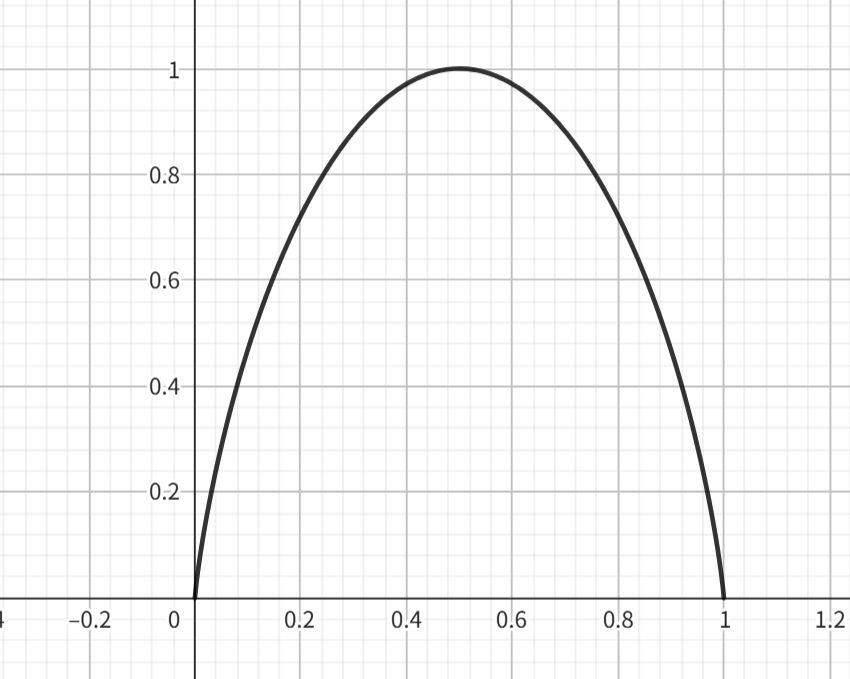
\includegraphics[width=.6\textwidth]{images/c2_1.png}
%     \caption{$H=x\log 1/x + (1-x)\log 1/(1-x)$的图像}
% \end{figure}